\documentclass[tikz]{standalone}
% B A C D E
% D C A E B
% rauzy induction after step 1
% A C D E
% C A E D
% rauzy induction after step 1'
% A C    D E
% C A    E D
\begin{document}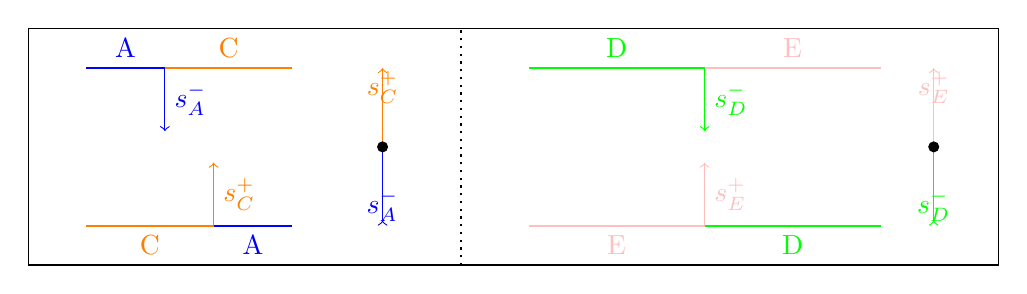
\begin{tikzpicture}
\draw (1.5, -1.5) rectangle (13.82,1.5);

\begin{scope}[xshift=6cm]
\draw[-<,blue] (0,0) -- node[near end] {$s_A^-$} (270:1);
\draw[->,orange] (0,0) -- node[near end] {$s_C^+$} (90:1);
\fill[black] (0,0) circle (2pt);
\end{scope}

\draw[dotted,thick] (7,-1.5) -- (7,1.5);

\begin{scope}[xshift=13cm]
\draw[->,pink] (0,0) -- node [near end] {$s_E^+$} (90:1);
\draw[-<,green] (0,0) -- node[near end] {$s_D^-$} (270:1);
\fill[black] (0,0) circle (2pt);
\end{scope}

\coordinate (t0) at (0,1);
\coordinate (t1) at (2.23606797749979, 1);
\coordinate (t2) at (3.23606797749979, 1);
\coordinate (t3) at (4.85410196624968, 1);


\coordinate (b0) at (0,-1);
\coordinate (b1) at (2.23606797749979, -1);
\coordinate (b2) at (3.85410196624968, -1);
\coordinate (b3) at (4.85410196624968, -1);

\begin{scope}[xshift=2cm]
\coordinate (tt3) at (5.85410196624968, 1);
\coordinate (t4) at (8.09016994374947, 1);
\coordinate (t5) at (10.32623792124926, 1);

\coordinate (bb3) at (5.85410196624968, -1);
\coordinate (b4) at (8.09016994374947, -1);
\coordinate (b5) at (10.32623792124926, -1);
\end{scope}

\draw[thick,blue] (t1) -- node[above] {A} (t2);
\draw[thick,orange] (t2) -- node[above] {C} (t3);
\draw[thick,green] (tt3) -- node[above] {D} (t4);
\draw[thick,pink] (t4) -- node[above] {E} (t5);
j
\draw[thick,orange] (b1) -- node[below] {C} (b2);
\draw[thick,blue] (b2) -- node[below] {A} (b3);
\draw[thick,pink] (bb3) -- node[below] {E} (b4);
\draw[thick,green] (b4) -- node[below] {D} (b5);

\draw[->,orange] (b2) -- node[right] {$s^+_C$} +(0,0.8);
\draw[->,pink] (b4) -- node[right] {$s^+_E$} +(0,0.8);

\draw[->,blue] (t2) -- node[right] {$s^-_A$} +(0,-0.8);
\draw[->,green] (t4) -- node[right] {$s^-_D$} +(0,-0.8);

%% saddle connections
%\fill[black] (0,-1) circle (2pt);
%\fill[black] (0,1) circle (2pt);
%\draw[green] (0,-1) -- node[right] {$s^+_D$} (0,0);
%\draw[red] (0,1) -- node[right] {$s^-_B$} (0,0);
%
%\fill[black] (.8,-1) circle (2pt);
%\fill[black] (.8,1) circle (2pt);
%\draw[blue] (.8,-1) -- node[right] {$s^+_A$} (.8,0);
%\draw[orange] (.8,1) -- node[right] {$s^-_C$} (.8,0);

\end{tikzpicture}\end{document}
